\begin{figure}

\centering

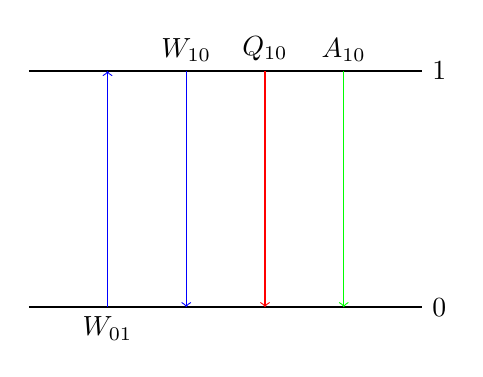
\begin{tikzpicture}

% Lower state
\draw [thick] ( 0, 0 ) -- ++( 5, 0 );

% Upper state
\draw [thick] ( 0, 3 ) -- ++( 5, 0 );

% Transitions
\draw [blue, ->] ( 1, 0 ) -- ++( 0, 3 );
\draw [blue, ->] ( 2, 3 ) -- ++( 0, -3 );
\draw [red, ->] ( 3, 3 ) -- ++( 0, -3 );
\draw [green, ->] ( 4, 3 ) -- ++( 0, -3 );

\node at ( 5, 0 ) [right] {0};
\node at ( 5, 3 ) [right] {1};

\node at ( 1, 0 ) [below] {\(W_{01}\)};
\node at ( 2, 3 ) [above] {\(W_{10}\)};
\node at ( 3, 3 ) [above] {\(Q_{10}\)};
\node at ( 4, 3 ) [above] {\(A_{10}\)};

\end{tikzpicture}

\caption[Transitions in a basic two-level model]{The figure shows energy levels and transitions between two levels, labeled 0 and 1, in a basic model of laser-induced fluorescence. Stimulated absorption and emission are shown in \textcolor{blue}{blue}, collisional quenching is shown in \textcolor{red}{red} and spontaneous emission is shown in \textcolor{green}{green}.}

\label{fig:twoLevel}

\end{figure}

